\section*{Annexes}

\subsection*{Annexe A - \textit{Clustering}}
Le partitionnement de données (ou \textit{data clustering}) est une des méthodes d'analyse des données. Elle vise à diviser un ensemble de données en différents «~paquets~» (ou \textit{clusters}) homogènes, en ce sens que les données de chaque sous-ensemble partagent des caractéristiques communes. Cela est matérialisé par des distances entre les objets manipulés. Davantage d'informations sur les différents algorithmes sont disponibles sur ce site~: \href{https://scikit-learn.org/stable/modules/clustering.html}{https://scikit-learn.org/stable/modules/clustering.html}.
\label{clustering}
\newpage

\subsection*{Annexe B - Résultats détaillés de la tentative de hierarchisation automatique du référentiel des métadonnées de l'Insee}

\begin{figure}[H]
    \centering
    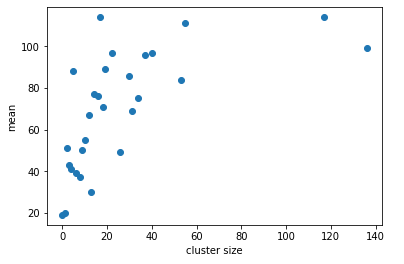
\includegraphics{images/hierarchisation-plot.png}
    \caption{Moyenne du nombre de mots dans les définitions sur un cluster en fonction de sa taille}
    \label{fig:hierarchisation}
\end{figure}

\begin{itemize}
    \item \textbf{Algorithme}~: \textit{Agglomerative Clustering}
    \item \textbf{Hyperparamètres}~: 
    \begin{itemize}
        \item Nombre de clusters~: 100
        \item Méthode d'agglomération~: \textit{complete} (minimise la distance entre les clusters)
        \newline
    \end{itemize}
\end{itemize}

On remarque assez nettement que les grands clusters sont composés principalement de concepts ayant des définitions longues, contrairement aux petits clusters où la longueur des définitions est plus variée. L'analyse de l'écart-type du nombre de mots par définitions pour les deux grands clusters confirme cette hypotèse, puisqu'ils sont respectivement de 21 mots pour le cluster de 117 concepts, et de 18 mots pour le cluster de 138 concepts.

\label{hierarchisation}
\newpage

\subsection*{Annexe C - Exemple de publication au format XML (extrait)}
\begin{lstlisting}[language=XML, basicstyle=\small]
<?xml version="1.0" encoding="UTF-8" standalone="yes" ?> 
<publication-sans-sommaire afficher-sommaire="true" afficher-sommaire-documentation="false">
  <titre>La pollution de l'air due au trafic automobile augmente les admissions aux urgences pour 
  maladies respiratoires </titre> 
  <auteur>Alexandre Godzinski (CGDD), Milena Suarez Castillo, division Marchés et entreprises 
  (Insee)</auteur> 
  <numero>46</numero> 
  <chapo>
    <paragraphe>
        La pollution de l'air issue du trafic automobile affecte la santé respiratoire des 
        populations urbaines à très court terme. Les perturbations dans les transports en commun 
        urbains un jour de grève permettent d'isoler des variations de pollution de l'air attribuables
        au trafic automobile. En cas de perturbation des transports en commun, une partie de la 
        population se tourne vers le transport automobile : les temps de parcours sont alors plus longs, 
        et la pollution de l'air augmente.
    </paragraphe> 
    <paragraphe>
        Le jour de la perturbation, la concentration en monoxyde de carbone est plus élevée.
        En conséquence, les admissions aux urgences pour affections aigues des voies respiratoires 
        supérieures sont significativement plus nombreuses. Les jours suivants, la concentration en 
        particules fines dans l'air augmente, ainsi que les admissions aux urgences pour 
        anomalies de la respiration.
    </paragraphe> 
    <paragraphe>
        À l'inverse, la perturbation dans les transports induit une moindre propagation
        virale, due à moins d'échanges et contacts entre individus. Les admissions aux urgences 
        pour grippe et gastro-entérite diminuent les jours suivant la perturbation. Ainsi, les 
        pathologies respiratoires d'origine virale seraient soumises à deux phénomènes aux effets 
        opposés qu'il importe de distinguer : une hausse induite par la pollution de l'air accrue, 
        une baisse du fait d'une moindre contagion. Au total, le constat d'une hausse des 
        admissions de certaines pathologies respiratoires confirme le rôle néfaste de la pollution
        de l'air sur la santé respiratoire.
    </paragraphe> 
  </chapo>
  <blocs>
    <bloc>
        <intertitre niveau="1">
            Établir un lien de cause à effet entre la pollution de l'air et 
            les admissions aux urgences pour cause respiratoire
        </intertitre> 
    </bloc>
    <bloc>
        <paragraphes>
            <paragraphe> 
                Dans les plus grandes aires urbaines    françaises, les seuils d'exposition au-delà desquels 
                la pollution est considérée comme nuisible par l'organisation mondiale de la santé (OMS) 
                sont très souvent dépassés [<lien-externe url="https://www.who.int/airpollution/data/cities/en/">
                base de données de l'OMS, 2018</lien-externe>]. En particulier, la pollution de l'air 
                issue du trafic automobile peut avoir des conséquences néfastes à très court 
                terme sur la santé des habitants. L'analyse des effets directs et indirects d'un événement 
                ponctuel, comme une perturbation dans les transports en commun un jour de grève, 
                permet ici d'établir un lien de cause à effet entre la pollution issue du trafic automobile et
                les admissions aux urgences pour certaines pathologies respiratoires. 
            </paragraphe>
        </paragraphes>
    </bloc>
    <bloc>
        <intertitre niveau="1">Une expérience naturelle : des transports en commun perturbés un jour de
        grève</intertitre> 
    </bloc>
  </blocs>
  <sources>
    <source>
        <blocs>
            <bloc>
                <paragraphes>
                    <paragraphe>
                    L'étude porte sur les dix plus grandes aires urbaines françaises (Paris, Lyon, Marseille,
                    Toulouse, Bordeaux, Lille, Nice, Nantes, Strasbourg, Rennes) sur la période 2010-2015, 
                    hors vacances scolaires.
                    </paragraphe> 
                <paragraphe>
            </bloc>
        </blocs>
    </source>
  </sources>
  <definitions>
    <definition id="definition-1">
        <blocs>
            <bloc>
                <paragraphes>
                    <paragraphe>
                    Un <emphase-normale>polluant primaire</emphase-normale> 
                    est un polluant directement émis par une source donnée, tandis qu'un 
                    <emphase-normale>polluant secondaire</emphase-normale> 
                    se forme par réaction dans l'atmosphère à partir d'autres polluants (l'ozone par exemple). 
                    </paragraphe>
                </paragraphes>
            </bloc>
        </blocs>
    </definition>
  </definitions>
</publication-sans-sommaire>
 
\end{lstlisting}
\label{publication-xml}
\newpage

\subsection*{Annexe D - Récapitualif et exemples de traitements}

Pharse d'exemple, tirée du \href{https://www.nytimes.com/2019/08/26/world/europe/g7-live-updates.html?action=click&module=Top\%20Stories&pgtype=Homepage}{New York Time} \cite{sent-ex}~:

\textit{«~President Trump sounded a positive note after taking a call from Chinese officials, and said he had given his blessing to Iran’s foreign minister holding meetings in Biarritz.~»}

\begin{figure}[H]
    \centering
    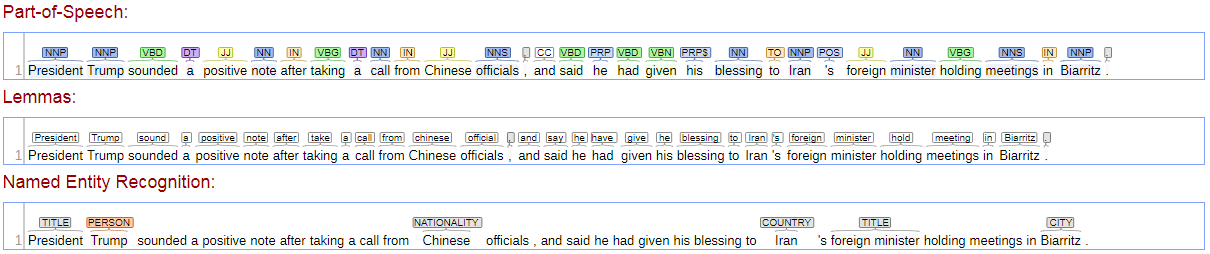
\includegraphics[scale=0.50]{images/nlp-recap-1.png}
    \caption{Récapitulatif des traitements NLP - \textit{POS}, \textit{Lemmatisation}, \textit{NER}}
    \label{fig:nlp-recap-1}
\end{figure}

\begin{figure}[H]
    \centering
    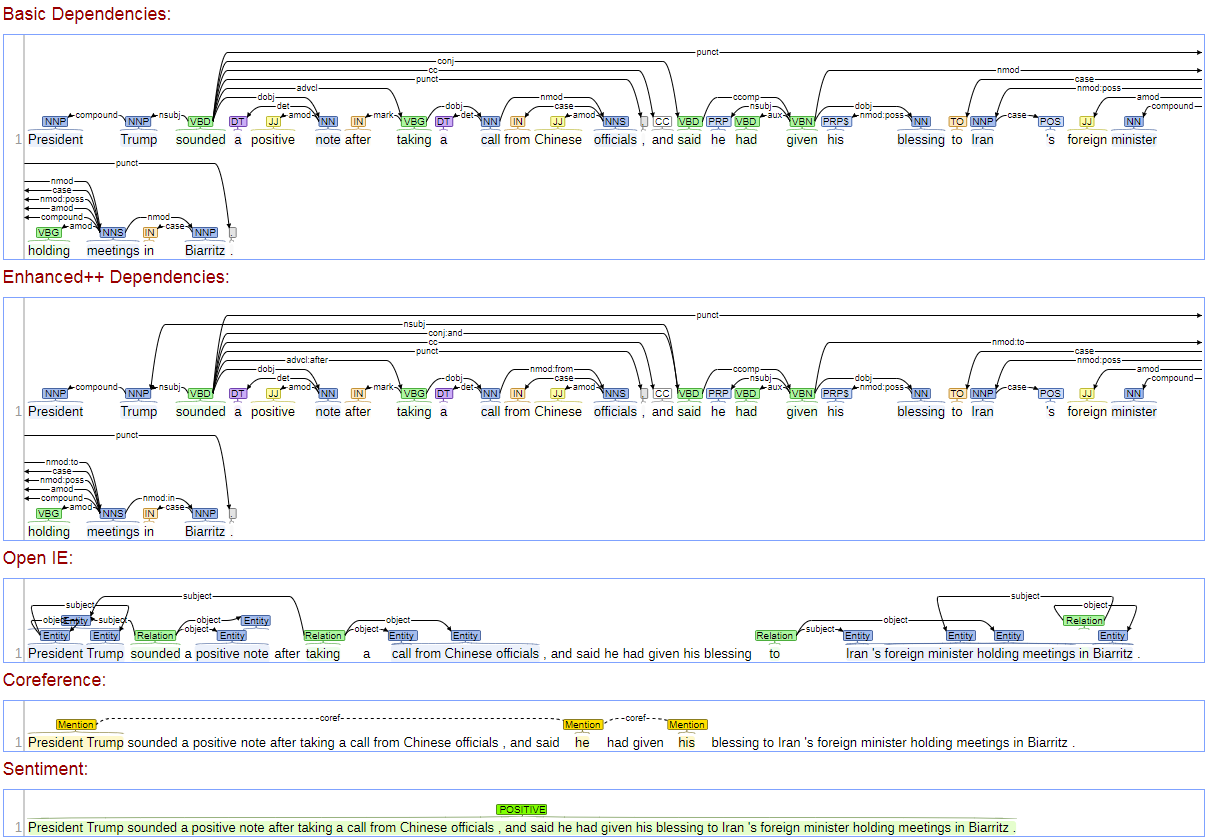
\includegraphics[scale=0.50]{images/nlp-recap-2.png}
    \caption{Récapitulatif des traitements NLP - \textit{Dependencies}, \textit{Open IE}, \textit{Coreference resolution}, \textit{Sentiment Analysis}}
    \label{fig:my_label}
\end{figure}

Les exemples ont été donnés à partir de la \href{http://corenlp.run/}{démonstration en ligne} \cite{corenlp-demo} de Stanford Core NLP. Des \href{https://explosion.ai/demos/}{démonstrateurs pour SpaCy} \cite{spacy-demo} sont également disponibles.
\newpage

\subsection*{Annexe E - Exemple de règles de reconnaissance d'entités nommées}

Exemples de règles pour le concept «~Salaire~».
\subsubsection*{Stanford Core NLP}
\begin{lstlisting}
{ 
    ruleType: "tokens", 
    pattern: ([{tag:"NOUN"} & {lemma:"salaire"}][{tag:"ADJ"}]*), 
    action: (Annotate(\$0, ner, "STAT-CPT"), 
            Annotate(\$0, mention, "http://id.insee.fr/concepts/definition/c1211")), 
    result: "STAT-CPT"
}
\end{lstlisting}

\subsubsection*{SpaCy}
\begin{lstlisting}
{ 
    "id": "c1211", 
    "label": "STAT-CPT", 
    "pattern": [{"POS": "NOUN", "lemma": "salaire"}, {"POS": "ADJ", "OP": "*"}] 
}
\end{lstlisting}

\label{rule-exemple}
